\documentclass[10pt,onecolumn]{article}

\usepackage{graphicx}

\usepackage{listings}
\lstset{
  captionpos=b,
  frame=single,
  numbers=left
}

\begin{document}

\title{Communicating between the kernel and \\ user-space in Linux using Netlink Sockets: \\ Source code reference}
\author{}
\date{}
\maketitle

\section{PROGRAMMING NETLINK SOCKETS}
\subsection{Netlink sockets from kernel-space}
We have coded a simple Linux kernel module that implements Netlink support to print the "Hello world" message when it receives a message from user-space.

We use the Listing. \ref{listing} as reference to start explaining the steps that you have to follow to add a new Netlink-based interface, that are:

\begin{enumerate}
  \item Reserve a Netlink bus for your new kernel subsystem: you have to edit \textit{include/linux/netlink.h} to add your Netlink bus. You may also include the bus definition in your code to avoid the bus definition in your code to avoid modifying the Linux kernel source code (lines 7-9).
  \item Include the appropriate header (lines 1-5), in particular it is important to include the headers that define the prototype of the functions required to register a new Netlink subsystem (lines 3-5) that are the generic BSD socket infrastructure (line 3), the generic network socket buffer (line 4) and the Netlink definitions and prototypes (line 5).
  \item Call \textit{netlink\_kernel\_create()} in the module initialization path to create the Netlink kernel socket: you have to pass a callback that is invoked when your new Netlink bus receives a message from user-space (see line 23-28). The function \textit{netlink\_kernel\_create()} returns a pointer to the \textit{sock} structure, which is used to store the kernel part of a generic BSD socket.
  \item Call \textit{netlink\_kernel\_release()} in the module exit path, which is executed when the Linux kernel module is removed to unregister the given Netlink socket bus (lines 38).
\end{enumerate}

\begin{lstlisting}[language=C, caption=Simple Netlink kernel module, label=listing1]
#include <linux/kernel.h>
#include <linux/module.h>
#include <net/sock.h>
#include <linux/skbuff.h>
#include <linux/netlink.h>

#ifdef NETLINK_EXAMPLE 21
#define NETLINK_EXAMPLE 21
#endif

#define NLEX_GRP_MAX 0

static struct sock *nlsk;

static void
nl_callback(struct sk_buff *skb)
{
    printk("Hello world\n");
}

static int __init nlexample_init(void)
{
    nlsk = netlink_kernel_create(&init_net,
                                 NETLINK_EXAMPLE,
                                 NLEX_GRP_MAX,
                                 nl_callback,
                                 NULL,
                                THIS_MODULE);

    if (nlsk == NULL)
    {
        printk(KERN_ERR "Can't create netlink\n");
        return -ENOMEM;
    }

    return 0;
}

void __exit nlexample_exit(void)
{
    netlink_kernel_release(nlsk);
}

module init(nlexample_init);
module exit(nlexample_exit);
\end{lstlisting}

Note that our example that we have represented in Listing. \ref{listing} registers no multicast groups (see constant NLEX\_GRP\_MAX which has been set to zero in line 11) that has been as a parameter to \textit{netlink\_kernel\_create()} in lines 23-28).

Using Netlink to print some output when a message is received is a good starting point, but it is not very useful. For that reason, we present a new example that exposes the variable \textit{myvar} to user-space by means of Netlink in Listing. \ref{listing} and Listing. \ref{listing}. This example supports two new operations: a) update the value of \textit{myvar} and b) get the current value of \textit{myvar}.

\begin{figure}[h]
\begin{center}
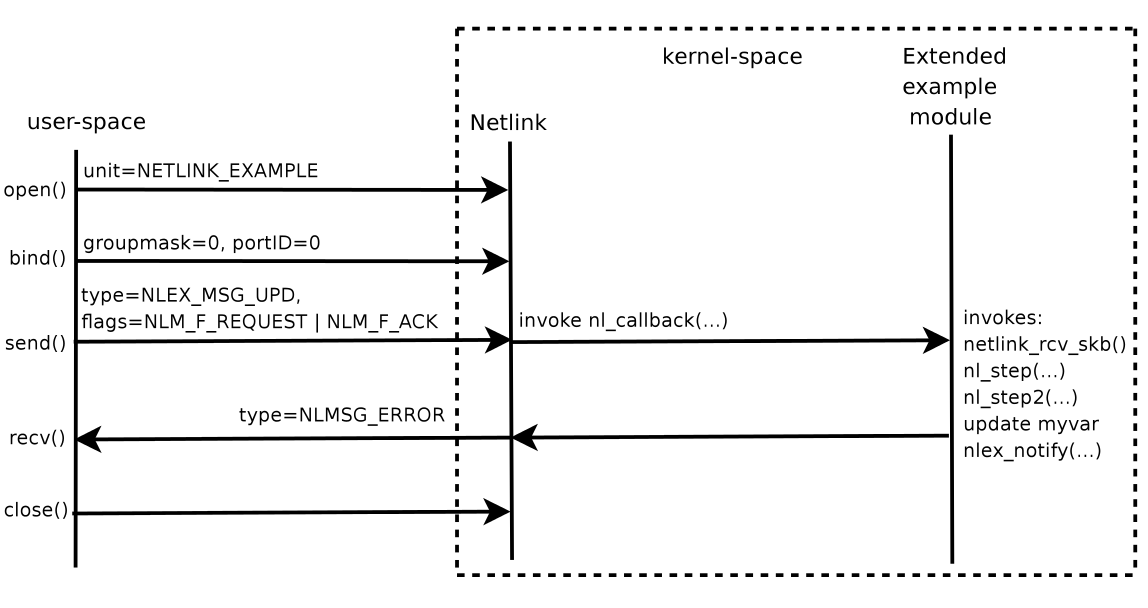
\includegraphics[height=5cm]{figure/netlink_update_sequence.png}
\end{center}
\caption{Update of the variable \textit{myvar} via Netlink}
\label{fig:netlink_update_sequence}
\end{figure}

In Figure \ref{fig}, we have represented the sequence diagram of an update of the variable \textit{myvar}. With regards to coding, we initially have to declare these two new actions in the header file of the Linux kernel module in Listing. \ref{listing}.

\begin{lstlisting}[language=C, caption=Example header file, label=listing2]
#ifndef _NLEXAMPLE_H_
#define _NLEXAMPLE_H_

#ifndef NETLINK_EXAMPLE
#define NETLINK_EXAMPLE 21
#endif

enum nlexample_msg_types {
    NLEX_MSG_BASE = NLMSG_MIN_TYPE,
    NLEX_MSG_UPD = NLEX_MSG_BAS,
    NLEX_MSG_GET,
    NLEX_MSG_MAX
};

enum nlexample_attr {
    NLE_UNSPEC,
    NLE_MYVAR,
    /* add your new attributes hew */
    __NLE_MAX,
};
#define NLE_MAX (__NLE_MAX - 1)

#define NLEX_GRP_MYVAR (1 << 0)
#endif
\end{lstlisting}

This list contains the following sections that are:

\begin{enumerate}
  \item The Netlink bus that we are going to register our new Netlink subsystem (lines 4-6), as we previously did in our "Hello World" example.
  \item The definition of supported actions (lines 8-13): the actions are mapped to Netlink message types starting by 16 to skip the reserved control message types from 0 to 15. We have defined NLEX\_MSG\_UPD to update the value of \textit{myvar}, and NLEX\_MSG\_GET to obtain the current value.
  \item The definition of the attribute type (lines 15-20): we have defined the attribute NLE\_MYVAR which can be used to store the new value of \textit{myvar} in the TLV Netlink payload. This new attribute can be used in messages going from user to kernel-space to set the new value of \textit{myvar}, but it can also be used to encapsulate the value of my \textit{myvar} for messages going from kernel to user-space as a result of a request to obtain the current value.
  \item The definition of the only multicast group supported by this example (NLEX\_GRP\_MYVAR in line 23) that allows you to subscribe to event notifications of changes in \textit{myvar}.
\end{enumerate}

In Listing. \ref{listing}, we have replaced the \textit{nl\_callback()} function that we have previously shown in Listing 1 (line 16) to support the new actions defined in Listing.

\begin{lstlisting}[language=C, caption=Extending the nl\_callback function, label=listing2]
static const
struct nla_policy nlex_policy[NLEMAX+1] = {
    [NLE_MYVAR] = { .type = NLA_U32},
};

static int
nl_step(struct sk_buff *skb,
        struct nlmsghdr *nlh)
{
    int err;
    struct nlattr *cda[NLE_MAX+1];
    struct nlattr *attr = NLMSG_DATA(nlh);
    int attrlen = nlh->nlmsg_len - NLMSG_SPACE(0);

    if (security_netlink_recv(skb, CAP_NET_ADMINI))
        return -EPERM;

    if (nlh->nlmsg_len < NLMSG_SPACE(0))
        return -EINVAL

    err = nla_parse(cda, NLE_MAX,
                    attr, attrlen, nlex_policy);
    if (err < 0)
        return err;

    return nl_step2(cda);
}

static void
nl_callback(struct sk_buff *skb)
{
    netlink_rcv_skb(skb, &nl_step);
}
\end{lstlisting}

In this new version of \textit{nl\_callback()} (lines 29-33), we call \textit{netlink\_rcv\_skb()} (line 32) which is a generic function that is used to perform initial sanity checkings on the message received. This function also appropriately handles Netlink message batches coming from user-space. The sanity checkings consist of the following:

\begin{enumerate}
  \item Check if the message contains enough room for the Netlink header.
  \item Check if the NLM\_F\_REQUEST flag has been set, which is used to tell that this message is going from user to kernel-space.
  \item Skip control messages if they are sent from user-space: Netlink replies with an acknowledgment message in this case. User-space applications do not usually send control messages to user-space.
  \item Check if the NLM\_F\_ACK flag has been set, in that case, the user-space process has explicitly requested an acknowledgment from kernel-space to make sure that the request has been performed successfully.
\end{enumerate}

Once the sanity checkings have been passed, the \textit{netlink\_rcv\_skb()} function invokes the callback function passed as an argument, which we have called \textit{nl\_step()} (lines 6-27 in Listing. \ref{listing}). The \textit{nl\_step()} function initially performs further non-generic sanity checkings, one of them to ensure that only user-space process with CAP\_NET\_ADMIN capabilities (that is, the process can perform network administrative tasks. Generally speaking, processes that run as superuser have this capability) (lines 15-16) can send messages to kernel-space. Then we proceed to parse the payload of the Netlink message that contains the attributes in TLV format. In order to perform the payload parsing, we use \textit{nla\_parse()} which takes an array of pointers to the Netlink attributes (see lines 21-22), whose size is the maximum number of attributes plus one (line 11), and updates the array to allow easy access to the attributes. The parsing includes the data validation to ensure that the data type stored in the attribute payload is correct (line 22, fifth parameter). This is done by means of a structure that defines the correspondence between the type stored in the attribute payload and the attribute type (lines 1-4). If there are problems in the parsing, an error is reported to user-space.

Once the parsing has been done, we call the function \textit{nl\_step2()} (line 26) which is implemented in Listing. \ref{listing}.

\begin{lstlisting}[language=C, caption=nl\_step2() function, label=listing3]
static int myvar;

static int
nl_step2(struct nlattr *cda[],
         struct nlmsghdr *nlh)
{
    int echo = nlh->nlmsg_flags & NLM_F_ECHO;
    int pid = nlh->nlmsg_pid;

    switch(nlh->nlmsg_type) {
        case NLEX_MSG_UPD:
            if (!cda[NLE_MYVAR])
                return -EINVAL;

            myvar = nla_get_u32(cda[NLEMYVAR]);
            nlex_notify(echo, pid);
            break;
        case NLEX_MSG_GET;
            nlex_unicast(pid);
            break;
    };
    return 0;
}
\end{lstlisting}

This function takes the array of Netlink attributes and it handles the message depending on its type according to the two possible actions that we have already defined in Listing. \ref{listing}. We handle the message depending on its type, that can be:

\begin{itemize}
  \item NLEX\_MSG\_UPD: we check if the NLE\_MYVAR attribute is set (lines 12-13), in that case, it takes the 32-bit value and it updates \textit{myvar} (line 15). Otherwise, it returns \textit{invalid argument} (EINVAL) to report a malformed message since a mandatory attribute is missing.
  \item NLEX\_MSG\_GET: it creates and delivers Netlink message to user-space containing the current value of \textit{myvar} via unicast. We have implemented the unicast deliver by means of the function \textit{nlex\_unicast()}, which is implemented in Listing. \ref{listing}.
\end{itemize}

The NLEX\_MSG\_UPD command also notifies to user-space listeners that the value of \textit{myvar} has changes (line 16 in Listing. \ref{listing}). This event notification is implemented by means of the  \textit{nlex\_notify()} function in Listing. \ref{listing}.

\begin{lstlisting}[language=C, caption=Broadcast notification of changes in myvar, label=listing5]
static int
nlex_notify(int rep, int pid)
{
    struct sk_buff *skb;

    skb = nlmsg_new(NLMSG_DEFAULT_SIZE, GFP_KERNEL);
    if (skb == NULL)
        return -ENOMEM;

    nlmsg_put(skb, pid, rep, NLEX_MSG_UPD, 0, 0);
    NLA_PUT_U32(skb, NLE_MYVAR, myvar);

    nlmsg_notify(nlsk, skb, pid,
                 NLEX_GRP_MYVAR,
                 rep, GRP_KERNEL);
    return 0;
nla_put_failure:
    return -1;
}
\end{lstlisting}

This function allocates memory for the Netlink message that will be send to the user-space listeners that are subscribed to the NLEX\_GRP\_MYVAR group. The message is stored in a network buffer of one memory page size (NLMSG\_DEFAULT\_SIZE is the size of one memory page minus the header of a Netlink message) for performance reasons (line 6).

We use the function \textit{nlmsg\_put()} to add the netlink header (line 10) and the NLA\_PUT\_U32() macro to add the value of \textit{myvar} in TLV format as the payload of the Netlink message (line 11). To deliver the Netlink message, we use \textit{nlmsg\_notify()} which sends notifications to all user-space listeners that are subscribed to the Netlink multicast group that alerts about changes in \textit{myvar}.

This function includes the Port-ID in the message (third parameter, line 13) to report other listeners that this change was triggered by another user-space process with that Port-ID. The multicast group is also passed (line 14) to tell Netlink to what multicast group it has to deliver the change report.

In Listing. \ref{listing6}, we have implemented \textit{nlex\_unicast} which performs the allocation (lines 6-8), building (lines 10-11) and delivery (line 13) of a Netlink message via unicast as response to a request to get the current value of \textit{myvar} (NLEX\_MSG\_GET message).

\begin{lstlisting}[language=C, caption=Unicast delivery to obtain the value of \textit{myvar}, label=listing6]
static int
nlex_unicast(int pid)
{
    struct sk_buff *skb;

    skb = nlmsg_new(NLMSG_DEFAULT_SIZE, GFP_KERNEL);
    if (skb == NULL)
        return -ENOMEM;

    nlmsg_put(skb, pid, rep, NLEX_MSG_UPD, 0, 0);
    NLA_PUT_U32(skb, NLE_MYVAR, myvar);

    nlmsg_unicast(nlsk, skb, pid);

    return 0;
nla_put_failure:
    return -1;
}
\end{lstlisting}

\subsection{Netlink sockets in user-space}
Netlink sockets are implemented on top of the generic BSD sockets interface. Thus, programming Netlink sockets in user-space is similar to programming common TCP/IP sockets.

In order to simplify the work with Netlink sockets, we propose in this work the use of \textit{libmnl}, written in C, which is a minimalistic user-space Netlink library oriented to Netlink developers.

There are other existing user-space Netlink libraries like:

\begin{itemize}
  \item \textit{libnl} is a complete library, also written in C, that aims to simplify the work with Netlink sockets. The development was started 2003 by Thomas Graf, it is currently the recommended library in the Linux kernel documentation. It provides an object-oriented abstraction layer to forget about Netlink sockets details. Thus, obtaining information from Netlink kernel subsystems is fairly easy and it allows very rapid application development for non-Netlink developers. This library hides many details of Netlink, for the purpose of this work, we have preferred to focus on a library that adds very few abstractions.
\end{itemize}

\subsection{Netlink sockets in user-space using libmnl}

We have written two user-space programs using the \textit{libmnl} library for our example Linux kernel module that we have exposed, they are:

\begin{itemize}
  \item \textit{change.c} that is used to change the current value of \textit{myvar}, the sequence diagram of this program is represented in Figure. \ref{fig} and the implementation in Listing \ref{listing7}.
  \item \textit{event.c} which allows to listen to asynchronous event notification that report changes in the \textit{myvar} value. This program is available in Listing. \ref{listing8}. In Figure. \ref{fig}, we have represented the sequence diagram of the asynchronous event notification.
\end{itemize}

\begin{lstlisting}[language=C, caption=\textit{change.c} program, label=listing7]
#include <stdio.h>
#include <stdlib.h>
#include <unistd.h>

#include <libmnl/libmnl.h>

#include "nlexample.h"

int main(void)
{
    char buf[getpagesize()];
    struct nlmsghdr ∗nlh;
    struct mnl_socket ∗nl;
    int ret, numbytes;
    unsigned int seq, oper;

    nlh = mnl_nlmsg_put_header(buf);
    nlh−>nlmsgtype = NLEX_MSG_UPD;
    nlh−>nlmsgflags = NLM_F_REQUEST | NLM_F_ACK;
    nlh−>nlmsgseq = seq = time(NULL);

    mnl_attr_put_u32(nlh ,NLE_MYVAR, 10);

    numbytes = mnl_nlmsg_getlen(nlh);

    nl = mn_socket_open(NETLINK_EXAMPLE);
    if (nl == NULL) {
        perror("mnl_socket_open");
        exit(EXIT_FAILURE);
    }

    ret = mn_socket_bind(nl, 0, 0);
    if (ret == −1) {
        perror("mnl_socket_bind");
        exit(EXIT_FAILURE);
    }

    ret = mnl_socket_sendto(nl, nlh, numbytes);
    if (ret == −1) {
        perror("mnl_socket_send");
        exit(EXIT_FAILURE);
    }

    ret = mnl_socket_recvfrom(nl, buf, sizeof(buf));
    if (ret == −1) {
        perror("recvfrom");
        exit(EXIT_FAILURE);
    }

    ret = mnl_cb_run(buf, ret, seq, NULL, NULL);
    if (ret == −1) {
        perror ("callback");
        exit(EXIT_FAILURE ) ;
    }
    mnl_socket_close(nl);
}
\end{lstlisting}

In Listing \ref{listing7}, we initially reserve room (line 17) for the Netlink header in a large enough buffer that we have previously allocated in the stack (line 11). Then, we fill the Netlink header fields with the message type, flags and sequence number (lines 18-20). The message type (line 18) is NLEX\_MSG\_UPD in this case to tell the kernel module that this message contains an update for \textit{myvar}. With regards to the flags, we have set NLM\_F\_REQUEST which is mandatory for requests that go from user to kernel-space and NLM\_F\_ACK to ask for an explicit Netlink error message from kernel-space containing the result of the operation (0 in case of success, otherwise a standard errno value). Finally, to generate the sequence numbering (line 20), we have selected the function \textit{time()} which returns the seconds since 1970. The kernel uses the same sequence number in the acknowledgment and data replies, thus, the sequence number provides a way to identify that a given message comes as reply of certain request. Therefore, there is no need to use incremental sequence numbers.

Once we have filled the Netlink header, we proceed with the TLV-payload building. In our case, the payload is simple since it is only composed of one attribute, which is NLE\_MYVAR (line 22). This Netlink attribute contains the new value that we want to assign to the kernel-space variable \textit{myvar}.

Now, it is time to create an user-space Netlink socket to send the message that we have built to kernel-space. Basically, we open the Netlink socket (line 26), then bind it (line 32) to no multicast groups (second parameter, line 32) and use the automatic Port-ID selection facility by using zero (third parameter, line 32).

The Netlink message is sent to kernel-space (line 38). Since we have explicitly requested an acknowledgment, we wait for it (line 44). The Netlink message received is passed to the callback runqueue which returns -1 (line 50) and it sets errno appropriately in case of error. Then, the user-space Netlink socket is closed (line 55).

In Listing. \ref{listing8}, we have implemented the event subscription. Basically, we open an user-space Netlink socket (line 30) and bind it (line 36) to the multicast group NLEX\_GRP\_MYVAR (second parameter, line 36). Then, we wait to receive Netlink messages that contain updates of the variable (lines 41-48).

Once we receive a Netlink message, we pass it to the callback runqueue which invokes the \textit{data\_cb()} function (line 9-21). This function parses the TLV-based payload of the Netlink message (line 15) and it initializes an array of pointers that contain the address of the attributes (variable tb in line 15, second parameter). Thus, we can easily access the attributes to retrieve the value of the attribute and print it (lines 17-18).

\begin{lstlisting}[language=C, caption=\textit{event.c} program, label=listing8]
#include <stdio.h>
#include <stdlib.h>
#include <unistd.h>

#include <libmnl/libmnl.h>

#include "nlexample.h"

static int
data_cb(const struct nlmsghdr ∗nlh, void ∗data)
{
    struct nla_ttr ∗tb[NLE MAX+1];
    struct nla_ttr ∗attr;

    mnl_attr_parse(nlh, tb, NLE_MAX);
    if (tb[NLE_MYVAR])
        printf("myvar=%u\n",
               mnl_attrget_u32(tb[NLE_MYVAR]));

    return MNL_CB_OK;
}

int main(void)
{
    struct mnl_socket ∗nl;
    char buf[getpagesize()];
    struct nlmsghdr *nlh = (struct nlmsghdr *)buf;
    int ret;

    nl = mnl_socket_open(NETLINK_EXAMPLE);
    if (nl == NULL) {
        perror("mnl_socket_open");
        exit(EXIT_FAILURE);
    }

    if (mnl_socket_bind(nl, NLEX_GRP_MYVAR, 0) < 0) {
        perror("mn_socket_bind");
        exit(EXIT_FAILURE);
    }

    ret = mnl_socket_recvfrom(nl, buf, sizeof(buf));
    while (ret > 0) {
        ret = mnl_cb_run(buf, ret, 0, data_cb, NULL);
        if (ret < 0)
            break;
        ret = mnl_socket_recvfrom(nl, buf,
                                    sizeof(buf));
    }
    if (ret == -1) {
        perror("error");
        exit(EXIT_FAILURE)
    }

    mnl_socket_close(nl);

    return 0;
}
\end{lstlisting}

\section{PROGRAMMING GENETLINK}
This section provides an overview on the GeNetlink programming from both user and kernel-space.

\subsection{Programming GeNetlink from kernel-space}

We have ported the previous example Linux kernel module that uses Netlink to export the variable \textit{myvar} to use GeNetlink. To do so, we have defined two commands in Listing. \ref{listing}:

\begin{itemize}
  \item NLEX\_CMD\_UPD, that allows you to update the current value of \textit{myvar}.
  \item NLEX\_CMD\_GET, that is used to retrieve the current value of \textit{myvar} via unicast.
\end{itemize}

This command values are used in the command field in the GeNetlink header. With regards to the attribute definitions (lines 10-15), we use the same declarations described in our previous example in Section .

\begin{lstlisting}[language=C, caption=GeNetlink example header file, label=listing9]
#ifndef _NLEXAMPLE_H_
#define _NLEXAMPLE_H_

enum nlexample_msg_types {
    NLEX_MSG_UPD = 0,
    NLEX_MSG_GET,
    NLEX_MSG_MAX
};

enum nlexample_attr {
    NLE_UNSPEC,
    NLE_MYVAR,
    __NLE_MAX,
};
#define NLE_MAX (__NLE_MAX - 1)

#define NLEX_GRP_MYVAR (1 << 0)
#endif
\end{lstlisting}

In Listing. \ref{listing}, we show the structures that are required to register the new
GeNetlink family, they are:

\begin{enumerate}
  \item The GeNetlink family structure (lines 11-17) that includes the type of ID number (line 12) which is automatically set by GeNetlink since GENL\_ID\_GENERATE is used. Then, the unique string name that is \textit{nlex}, and the maximum number of TLV attributes that can contain the GeNetlink message (line 16). The version field (line 15) allows to declare different versions of the same family, this can be used in the future to introduce changes in the GeNetlink message format, and operations without breaking backward compatibility.
  \item The family operations (lines 23-32), that include the two commands supported. This structure links the command type (lines 25 and 29) with a callback function, which is the \textit{doit} field in the structure (lines 26 and 30). Thus, if a GeNetlink message for this family is received, it is passed to the appropriate callback.
  \item The family multicast group (lines 19-21), that is only one group in this case that is identified by the string name \textit{example}. This group allows user-space listeners to subscribe to asynchronous reports on changes in \textit{myvar}.
\end{enumerate}

\begin{lstlisting}[language=C, caption=GeNetlink example declarations, label=listing10]
#include <linux/kernel.h>
#include <linux/module.h>
#include <linux/skbuff.h>
#include <linux/genetlink.h>
#include <net/genetlink.h>

#include "genlexample.h"

static int myvar;

static struct genl_family genl_ex_family = {
    .id = GENL_ID_GENERATE,
    .name = "nlex",
    .hdrsize = 0,
    .version = 1,
    .maxattr = NLE_MAX,
};

static struct genl_multicast_group genl_ex_mc = {
    .name = "example",
};

static struct genl_ops genl_ex_ops [] = {
    {
        .cmd = NLEX_CMD_GET,
        .doit = genl_get_myvar,
    },
    {
        .cmd = NLEX_CMD_UPD,
        .doit = genl_upd_myva,
    },
};
\end{lstlisting}

The initialization consists of the registration of the new GeNetlink family (lines 5-7), the registration of the operations (lines 9-14) and the registration of the multicast group (lines 16-19).

\begin{lstlisting}[language=C, caption=GeNetlink family registration and unregistration routines, label=listing11]
static int __init nlexample_init(void)
{
    int i, ret = -EINVAL;

    ret = genl_register_family(&genl_ex_family);
    if (ret < 0)
        goto err;

    for (i = 0; i < ARRAY_SIZE(genl_ex_ops); i++) {
        ret = genl_register_ops(&genl_ex_family,
                                &genl_ex_ops[i]);
        if (ret < 0)
            goto err_unregister;
    }

    ret = genl_register_mc_group(&genl_ex_family,
                                 &genl_ex_mc);
    if (ret < 0)
        goto err_unregister;

    return ret;

err_unregister:
    genl_unregister_family(&genl_ex_family);
err:
    return ret;
}

void __exit nlexample_exit(void)
{
    genl_unregister_family(&genl_ex_family);
}

module_init(nlexample_init);
module_exit(nlexample_exit);
\end{lstlisting}

The operation to retrieve the current value of \textit{myvar} is implemented in the Listing. \ref{listing}. This function consists of the allocation of the Netlink message (lines 7-9), the initialization of the GeNetlink header (lines 11-12) and the addition of the TLV-based payload that contains the current value of the \textit{myvar} (line 14). Then, the GeNetlink message is delivered via unicast to the user-space process (line 16).

\begin{lstlisting}[language=C, caption=Get \textit{myvar} routine, label=listing12]
static int
genl_get_myvar(struct sk_buff *skb,
               struct genl_info *info)
{
    struct sk_buff *msg;

    msg = nlmsg_new(NLMSG_DEFAULT_SIZE, GFP_KERNEL);
    if (msg == NULL)
        return -ENOMEM;

    genlmsg_put(msg, info->snd_pid, info->snd_seq,
                &genl_ex_family, 0, NLEX_CMD_UPD);

    NLA_PUT_U32(msg, NLE_MYVAR, myvar);

    genlmsg_unicast(msg, info->snd_pid);

    return 0;

nla_put_failure:
    return -ENOBUFS;
}
\end{lstlisting}

The update of the value of \textit{myvar} via the example GeNetlink family is implemented in the Listing. \ref{listing}.

\begin{lstlisting}[language=C, caption=Update \textit{myvar} routine, label=listing13]
static int
genl_upd_myvar(struct sk_buff *skb,
               struct genl_info *info)
{
    struct sk_buff *msg;

    if (!info->attrs[NLE_MYVAR])
        return -ENIVAL;

    myvar = nla_get_u32(info->attrs[NLE_MYVAR]);

    msg = nlmsg_new(NLMSG_DEFAULT_SIZE, GFP_KERNEL);
    if (msg == NULL)
        return -ENOMEM;

    genlmsg_put(msg, info->snd_pid, info ->snd_seq,
                &genl_ex_family, 0, NLEX_CMD_UPD);

    NLA_PUT_U32(msg, NLE_MYVAR, myvar);

    genlmsg_multicast(msg, 0, genl_ex_mc.id,
                      GFP_KERNEL);
    return 0;

nla_put_failure:
    return -ENOBUFS;
}
\end{lstlisting}

Initially, this routine verifies that the message coming from user-space contains the NLE\_MYVAR attribute with the new \textit{myvar} value that user-space wants to set (lines 7-8). If the attribute is missing, the routine returns an error to report that the message is invalid since the NLE\_MYVAR attribute is mandatory. If the message contains the attribute, the routine updates the value of the variable \textit{myvar} (line 10). Since user-space process can subscribe to the example multicast to track changes in the myvar variable, this routine has to report the change in the variable. The reporting consists of allocating memory for the Netlink message (lines 12-14), filling the GeNetlink header (lines 16-17) with the Port-ID of the process that has changed the variable (second parameter), the same sequence number used in the message received from user-space (third parameter), the GeNetlink family (line 17, fourth parameter) and the Netlink message flags (fifth parameter) which are none in this case, and the command type of the message (sixth parameter). To conclude the message building, the routine adds the new value of \textit{myvar} in TLV format as payload of the GeNetlink message. Then, the message is delivered to the user-space listeners that are subscribed to the \textit{example} group (lines 21-22).

\subsection{Programming GeNetlink from user-space}

Since the family and multicast IDs are assigned in run-time, we initially have to look up for the IDs to send requests and to subscribe to GeNetlink multicast groups from user-space. For that task, we use a program that takes the GeNetlink family name as first parameter, it sends a request to the GeNetlink control family \textit{nlctrl} which is the only family with a fixed family ID, and it displays the family ID and the list of available multicast groups and their corresponding IDs. The body of the main() function of this resolver has been represented in Listing. \ref{listing14}.

\begin{lstlisting}[language=C, caption=GeNetlink family and multicast resolver, label=listing14]
#include <stdio.h>
#include <stdlib.h>
#include <unistd.h>

#include <libmnl/libmnl.h>
#include <linux/genetlink.h>

int main(int argc, char *argv[])
{
    struct mnl_socket *nl;
    char buf[getpagesize()];
    struct nlmsghdr *nlh;
    struct genlmsghdr *genl;
    int ret, numbytes, hdrsize;
    unsigned int seq;

    if (argc != 2) {
        printf("%s [family name]\n", argv[0]);
        exit(EXIT_FAILURE);
    }

    nlh = mnl_nlmsg_put_header(buf);
    nlh->nlmsg_type = GENL_ID_CTRL;
    nlh->nlmsg_flags = NLM_F_REQUEST | NLM_F_ACK;
    nlh->nlmsg_seq = seq = time(NULL);

    hdrsize = sizeof(struct genlmsghdr);
    genl = mnl_nlmsg_put_extra_header(nlh, hdrsize);
    genl->cmd = CTRL_CMD_GETFAMILY;
    genl->version = 1;

    mnl_attr_put_str_null(nlh,
                          CTRL_ATTR_FAMILY_NAME,
                          argv[1]);

    numbytes = mnl_nlmsg_get_len(nlh);

    nl = mnl_socket_open(NETLINK_GENERIC);
    if (nl == NULL) {
        perror("mnl_socket_open");
        exit(EXIT_FAILURE);
    }

    if (mnl_socket_bind(nl, 0, 0) < 0) {
        perror("mnl_socket_bind");
        exit(EXIT_FAILURE);
    }

    if (mnl_socket_sendto(nl, nlh, numbytes) < 0) {
        perror("mnl_socket_send");
        exit(EXIT_FAILURE);
    }

    ret = mnl_socket_recvfrom(nl, buf, sizeof(buf));
    while (ret > 0) {
        ret = mnl_cb_run(buf, ret, seq, data_cb, NULL);
        if (ret <= 0)
            break;
        ret = mnl_socket_recvfrom(nl, buf, sizeof(buf));
    }
    if (ret == -1) {
        perror("error");
        exit(EXIT_FAILURE);
    }
    mnl_socket_close(nl);

    return 0;
}
\end{lstlisting}

The resolver initially checks for the required family name as argument (lines 17-20). Then, it starts by building the Netlink header (lines 22-25) in which the message type is GENL\_ID\_CTRL that is the fixed ID of the GeNetlink control family. It follows the GeNetlink header building (lines 27-30) in which the command used to retrieve the GeNetlink family information is CTRL\_CMD\_GETFAMILY (line 29). The payload of the message is composed of one Netlink attribute that contains the GeNetlink family name that we want to retrieve information.

Then, we open the Netlink socket (lines 38-42) using the NETLINK\_GENERIC bus which corresponds GeNetlink. We bind it to no multicast groups (lines 44-47) and we finally send the message (lines 49-52). Then, we wait for the reply (line 54 and 59) and we handle the data received by means of the callback runqueue (line 56) which calls the function \textit{data\_cb()} to perform the interpretation of the reply. If no GeNetlink family was found, we receive a Netlink message that contains the ENOENT error (No such entry exists).

We have represented the function \textit{data\_cb()} in Listing. \ref{listing15}.

\begin{lstlisting}[language=C, caption=Digesting GeNetlink control messages, label=listing15]
static int
data_cb(const struct nlmsghdr *nlh, void *data)
{
    struct nlattr *tb[CTRL_ATTR_MAX+1];
    struct genlmsghdr *genl = 
          nml_nlmsg_get_data(nlh);

    mnl_attr_parse_at_offset(nlh, sizeof(*genl),
                             tb, CTRL_ATTR_MAX);
    if (tb[CTRL_ATTR_FAMILY_ID]) {
        printf("family-id:%d\n",
            mnl_attr_get_u16(tb[CTRL_ATTR_FAMILY_ID]));
    }
    if (tb[CTRL_ATTR_MCAST_GROUPS]) {
        printf("multicast->id\n");
        parse_mc_grps(tb[CTRL_ATTR_MCAST_GROUPS]);
    }

    return MNL_CB_OK;
}
\end{lstlisting}

This function parses the payload of the message (lines 8-9) and it sets the array of pointers to access the attributes. Then, we check if the family ID attribute is available in the message (line 10). If so, the routine displays the family ID (lines 11-12) which is required to fill the Netlink type to send a message for that family. Moreover, the routine parses the set of multicast groups that are available in the GeNetlink family (line 16).

The set of multicast groups available in a given family is stored in a three-level nesting. The first level uses the attribute type CTRL\_ATTR\_MCAST\_GROUPS, then the second level contains a set of attribute types starting by 1 to \textit{n}, where \textit{n} is the number of multicast groups available. Finally, the third level contains the attributes CTRL\_ATTR\_MCAST\_GRP\_NAME, which contains the multicast group name, and CTRL\_ATTR\_MCAST\_GRP\_ID, that is the ID of that given multicast group. We have represented the multicast group parsing in Listing. \ref{listing}.

\begin{lstlisting}[language=C, caption=Parsing GeNetlink multicast groups, label=listing16]
static void
parse_one_mc_group(struct nlattr *pos)
{
    struct nlattr *tb[CTRL_ATTR_MCAST_GRP_MAX+1];

    mnl_attr_parse_nested(pos, tb,
                          CTRL_ATTR_MCAST_GRP_MAX);
    if (tb[CTRL_ATTR_MCAST_GRP_NAME] &&
        tb[CTRL_ATTR_MCAST_GRP_ID]) {
        printf("\"%s\"->%d\n",
            mnl_attr_get(tb[CTRL_ATTR_MCAST_GRP_NAME]),
            mnl_attr_get_u32(tb[CTRL_ATTR_MCAST_GRP_ID]));
    }
}

static void
parse_mc_grps(struct nlattr *nested)
{
    struct nlattr *pos;
    int len;
    const char *mcast_grp_name;
    int mcast_grp_id;

    mnl_attr_for_each_nested(pos, nested, len)
     parse_one_mc_group(pos);
}
\end{lstlisting}

Basically, the function \textit{parse\_mc\_groups()} (lines 16-26) iterates over the second level of nested attributes (lines 24-25) and parses it by means of \textit{parse\_one\_mc\_groups()} (line 25). This function parses the attributes (lines 6-7) and it displays the multicast group name and the ID (lines 10-12).

Now that we have a program to obtain the GeNetlink family ID and the multicast group ID, we can implement the user-space support for our example GeNetlink Linux kernel module that we have previously represented in Listings. 9, 10, 11, 12 and 13. We have implemented the GeNetlink version of two programs that we have previously discussed in Section \ref{sec}, they are:

\begin{itemize}
  \item \textit{change.c} that can be used to update the \textit{myvar} variable. This program takes as first argument the GeNetlink family ID that we have obtained from the resolver.
  \item \textit{event.c} that allows to subscribe to events of our example GeNetlink family.
\end{itemize}

In Listing. \ref{listing17}, we show the implementation of the \textit{change.c} program. To update the \textit{myvar} variable, we initially build the Netlink header (lines 24-27), whose message type has been obtained by means of the resolve program and it has been passed as argument (line 25). It follows the GeNetlink header (lines 29-31) and the payload that contains the attribute NLE\_MYVAR that encapsulates the new value of \textit{myvar} that has been passed as second argument (line 33). Then, we open the Netlink socket (line 37) and bind it to no multicast groups (line 42) and send it (line 48). We wait for the reply from kernel-space (line 54) and pass the data received to the runqueue callback (line 60) to handle the acknowledgment received in return to inform about the operation success or failure. The routines ends by closing the Netlink socket (line 65).

\begin{lstlisting}[language=C, caption=change.c for GeNetlink, label=listing17]
#include <stdio.h>
#include <stdlib.h>
#include <unistd.h>

#include <libmnl/libmnl.h>
#include <linux/genetlink.h>

#include "genlexample.h"

int main(int argc, char *argv[])
{
    char buf[getpagesize()];
    struct nlmsghdr *genl;
    struct genlmsghdr *genl;
    struct mnl_socket *nl;
    int ret, hdrsize, numbytes;
    unsigned int seq, oper;

    if (argc != 3) {
        printf("%s [Family ID] [myvar]\n", argv[0]);
        exit(EXIT_FAILURE);
    }

    nlh = mnl_nlmsg_put_header(buf);
    nlh−>nlmsg_type = atoi(argv[1]);
    nlh−>nlmsg_flags = NLM_F_REQUEST | NLM_F_ACK;
    nlh−>nlmsg_seq = seq = time(NULL);

    mnl_attr_put_u32(nlh, NLE_MYVAR, atoi(argv[2]));

    numbytes = mnl_nlmsg_get_len(nlh);

    nl = mn_socket_open(NETLINK_GENERIC);
    if (nl == NULL) {
        perror("mnl_socket_open");
        exit(EXIT_FAILURE);
    }
    ret = mn_socket_bind(nl, 0, 0);
    if (ret == -1) {
        perror("mnl_socket_bind");
        exit(EXIT_FAILURE);
    }

    ret = mnl_socket_sendto(nl, nlh, numbytes);
    if (ret == -1) {
        perror("mnl_socket_send");
        exit(EXIT_FAILURE);
    }

    ret = mnl_socket_recvfrom(nl, buf, sizeof(buf));
    if (ret == -1) {
        perror("recvfrom");
        exit(EXIT_FAILURE);
    }

    ret = mnl_cb_run(buf, ret, seq, NULL, NULL);
    if (ret == -1) {
        perror ("callback");
        exit(EXIT_FAILURE ) ;
    }
    mnl_socket_close(nl);
}
\end{lstlisting}

We have represented the event subscription program in Listing. \ref{listing18}. This routine initially opens a Netlink socket (line 38) and it binds to no multicast groups (line 44). Since the common binding operation only allows to subscribe by means of a group mask (Thus, this allows to subscribe up to the limited number 32 groups.), we use the socket option NETLINK\_ADD\_MEMBERSHIP (lines 50-53) which allows to subscribe to a group by an integer. Thus, we can subscribe to any of the existing 2\textsuperscript{32} multicast groups. This multicast ID is passed as first argument to the program and it has been previously obtained by means of the \textit{resolve} program.

Once we are subscribed to the event reporting, we wait for event messages (lines 55 and 60) and we handle the messages received by means of the callback runqueue (line 57) that invokes the \textit{data\_cb()} function. This function parses the payload of the GeNetlink messages received (lines 17-18) and it displays the new value (lines 20-21).

\begin{lstlisting}[language=C, caption=event.c for GeNetlink, label=listing18]
#include <stdio.h>
#include <stdlib.h>
#include <unistd.h>

#include <libmnl/libmnl.h>
#include <linux/genetlink.h>

#include "genlexample.h"

static int
data_cb(const struct nlmsghdr *nlh, void *data)
{
    struct nlattr *tb[NLE_MAX+1];
    struct nlattr *attr;

    int hdrsize = sizeof(struct genlmsghdr);

    mnl_attr_parse_at_offset(nlh, hdrsize,
                             tb, NLE_MAX);
    if (tb[NLE_MYVAR])
        printf("myvar=%u\n",
               mnl_attrget_u32(tb[NLE_MYVAR]));

    return MNL_CB_OK;
}

int main(int argc, char *argv[])
{
    struct mnl_socket *nl;
    char buf[getpagesize()];
    struct nlmsghdr *nlh = (struct nlmsghdr *)buf;
    int ret, grp;

    if (argc != 2) {
        printf("%s GeNL_multicast_ID\n", argv[0]);
        exit(EXIT_FAILURE);
    }

    nl = mn_socket_open(NETLINK_GENERIC);
    if (nl == NULL) {
        perror("mnl_socket_open");
        exit(EXIT_FAILURE);
    }

    ret = mn_socket_bind(nl, 0, 0);
    if (ret == -1) {
        perror("mn_socket_bind");
        exit(EXIT_FAILURE);
    }

    grp = atoi(argv[1]);
    mnl_socket_setsocket(nl,
                         NETLINK_ADD_MEMBERSHIP,
                         &grp, sizeof(grp));

    ret = mnl_socket_recvfrom(nl, buf, sizeof(buf));
    while (ret > 0) {
        ret = mnl_cb_run(buf, ret, 0, data_cb, NULL);
        if (ret < 0)
            break;
        ret = mnl_socket_recvfrom(nl, buf, sizeof(buf));
    }
    if (ret == -1) {
        perror("error");
        exit(EXIT_FAILURE)
    }

    mnl_socket_close(nl);

    return 0;
}
\end{lstlisting}

\end{document}
